\documentclass[
  aps,
  prl,
  reprint,
  amsmath,
  amssymb,
  superscriptaddress,
  floatfix,
  nofootinbib
]{revtex4-2}

\usepackage{graphicx}
\usepackage{bm}
\usepackage{url}
\usepackage{color}
\usepackage[colorlinks=true,linkcolor=blue,citecolor=blue,urlcolor=blue]{hyperref}

\newcommand{\tenB}{$^{10}$B}
\newcommand{\elevenB}{$^{11}$B}
\newcommand{\kzero}{k_{0}}
\newcommand{\Tr}{\mathcal{T}}

\begin{document}

\title{Hyperuniform isotope engineering of phonon transport: exact scaling
laws and a stealthy transparency window in hexagonal boron nitride}

\author{Ronghua Wu}
\email{wrh@gdtzn.com}
\affiliation{Zhuhai Jiuchongtian Aviation Technology Co., Ltd., Zhuhai, China}
\author{Ruqing Chen}
\email{ruqing@hotmail.com}
\affiliation{GUT Geoservice Inc., Montreal, Canada}

\date{\today}

\begin{abstract}
Isotopic substitution is one of the few strictly mass-like perturbations
available in a crystal: within the Born--Oppenheimer approximation the
interatomic force constants are invariant under isotope exchange, so an
isotope pattern modifies the dynamical matrix through the mass factors alone.
This makes the \emph{spatial arrangement} of isotopes a design variable
independent of the isotopic variance $g_2$ that has been the sole focus of
isotope engineering to date. We generalize the Tamura theory of
phonon--isotope scattering to spatially correlated arrangements by introducing
the mass-fluctuation structure factor $S_\epsilon(\bm{k})=g_2\,s(\bm{k})$, and
show that when $s(k)\simeq(k/\kzero)^\alpha$ at small wavenumber the relaxation
rate obeys the exact scaling law $\tau_{\rm iso}^{-1}\propto\omega^{\,d+1+\alpha}$
in $d$ dimensions, with closed-form angular prefactor $2/(\alpha+2)$. The
hyperuniformity exponent therefore contributes an additive,
dimension-independent correction to the Rayleigh exponent, orthogonal to the
dimensional baseline. We realize the class~II case $\alpha=1$ using
sequences with Gaussian-unitary-ensemble spacing statistics---of which the
unfolded nontrivial zeros of the Riemann zeta function are the canonical
example---mapped onto a one-dimensional \tenB/\elevenB\ modulation of
hexagonal boron nitride, obtaining $\tau_{\rm iso}^{-1}\propto\omega^5$ in
place of the Rayleigh $\omega^4$. We further find numerically that sequences built
from zeros at finite height are more rigid than GUE, giving
$\alpha=1.49\pm0.12$, and that this exponent is independent of the height of
the zeros used: across eight disjoint windows spanning
$\bar\gamma=1.2\times10^{3}$ to $6.2\times10^{7}$ the fitted trend is
$-0.138\pm0.075$, consistent with zero, so the deeper suppression is available
without any tuning. For stealthy (class~I) arrangements we prove
that the golden-rule rate vanishes identically, not merely asymptotically, for
all $\omega<vK/2$, where $K$ is the stealthiness wavenumber. We propose a
differential transmission observable $\Delta\Tr(\omega)$ between
concentration-matched samples that cancels the Casimir and anharmonic
backgrounds to first order, identify a feasible observation window of
$4$--$7$~THz at liquid-helium temperature, and state the resulting fabrication
specification---$1.25$~nm modulation pitch over $300\,\mu$m---as an explicit
design target that exceeds present growth capability.
\end{abstract}

\maketitle

\section{Introduction}
\label{sec:intro}

Isotope engineering of phonon transport has, since the earliest work on
diamond and silicon, been organized around a single scalar, the mass variance
\begin{equation}
  g_2 = \sum_i f_i\left(1-\frac{m_i}{\bar m}\right)^{\!2},
  \label{eq:g2}
\end{equation}
with $f_i$ the abundance of isotope $i$. Reducing $g_2$ by isotopic
purification has produced record thermal conductivities in diamond, silicon,
boron arsenide, and most strikingly in cubic boron nitride, where enrichment
to $99\%$ in either boron isotope yields
$\kappa_{\rm RT}>1600~\mathrm{W\,m^{-1}K^{-1}}$~\cite{Chen2020}. In hexagonal
boron nitride the same strategy raises the in-plane conductivity to
$585~\mathrm{W\,m^{-1}K^{-1}}$~\cite{Yuan2019} and lengthens hyperbolic
phonon-polariton lifetimes substantially~\cite{Giles2018}.

All of this treats the isotope distribution as \emph{random}. The Tamura and
Klemens theories that underpin it assume explicitly that isotopic occupations
on distinct sites are uncorrelated~\cite{Tamura1983,Klemens1955}; under that
assumption the mass-fluctuation structure factor is white and the whole
problem collapses onto $g_2$.

There is no physical reason for this assumption to hold in a \emph{grown}
crystal. Layer-by-layer precursor switching permits, in principle, an
arbitrary prescribed sequence. This paper asks what becomes available once the
arrangement is treated as a design variable at fixed $g_2$.

The natural language is hyperuniformity. A point pattern is hyperuniform when
its structure factor vanishes in the infinite-wavelength limit, so that
long-wavelength density fluctuations are anomalously
suppressed~\cite{Torquato2018,Torquato2003}. Torquato's classification
organizes hyperuniform systems by the exponent $\alpha$ in $S(k)\sim|k|^\alpha$:
class~I ($\alpha>1$, all crystals and quasicrystals), class~II ($\alpha=1$,
logarithmically growing number variance~\cite{Zachary2009}), and class~III
($0<\alpha<1$); the connection between random-matrix spectra, number theory
and hyperuniform point processes is developed in
Ref.~\cite{Torquato2008}. Random
arrangements correspond to $\alpha=0$.

Long-wavelength phonons are sensitive to precisely the fluctuations that
hyperuniformity suppresses. We establish below that the isotope-scattering
exponent is controlled by $\alpha$ in a simple additive way.

To realize a specific $\alpha$ we require a sequence whose small-$k$ structure
factor is known exactly. The nontrivial zeros of the Riemann zeta function
provide the canonical example. Under the Montgomery--Odlyzko
correspondence~\cite{Montgomery1973,Odlyzko1987} the unfolded zeros have pair
statistics identical to the eigenvalues of the Gaussian unitary ensemble
(GUE), for which Dyson's exact solution yields the closed form
\begin{equation}
  s_{\rm GUE}(k)=
  \begin{cases}
    k/2\pi, & k<2\pi,\\[2pt]
    1,      & k\ge 2\pi,
  \end{cases}
  \label{eq:sgue}
\end{equation}
in units of unit mean spacing. This is $\alpha=1$, though only asymptotically in
the height of the zeros; Sec.~\ref{sec:discretization} quantifies the finite-height
departure, which is substantial at any realizable length.

We emphasize that the zeros enter purely as a mathematically exact generator
of a class~II sequence. Every prediction below depends on the arrangement only
through $\alpha$, and any $\beta=2$ level-repelling point process would serve
identically. The zeros are chosen because their structure factor is known in
closed form, not because of any presumed significance of the sequence itself.

\section{Theoretical framework}
\label{sec:theory}

\subsection{Exactness of the mass perturbation}

Within the Born--Oppenheimer approximation nuclear masses do not enter the
electronic Hamiltonian. The second-order force-constant tensor
\begin{equation}
  \Phi_{ij}^{\alpha\beta}
    = \frac{\partial^{2}E}{\partial u_i^\alpha\,\partial u_j^\beta}
  \label{eq:phi}
\end{equation}
is therefore invariant, element by element, under isotopic substitution; only
the mass factors in the dynamical matrix change,
\begin{equation}
  D(\bm q)=M^{-1/2}\,\Phi(\bm q)\,M^{-1/2}.
  \label{eq:dynmat}
\end{equation}

Two consequences follow. Physically, an isotope pattern probes the phonon
eigenvectors without deforming the potential-energy surface. Computationally,
$\Phi$ need be evaluated only once, on the primitive cell; arbitrary
arrangements follow at zero additional first-principles cost by permuting the
diagonal matrix $M$ (Sec.~\ref{sec:methods}).

Writing $M_n=\bar M(1+\epsilon_n)$ with $\epsilon_n\equiv\Delta M_n/\bar M$,
\begin{equation}
  \delta D = -\,\omega^{2}\sum_n \epsilon_n\,|n\rangle\langle n|
             + \mathcal{O}(\epsilon^{2}).
  \label{eq:deltaD}
\end{equation}
For the \tenB/\elevenB\ pair $|\epsilon|\lesssim0.05$, so second-order
contributions are suppressed by $\sim10^{-3}$ relative; their role is bounded
in Sec.~\ref{sec:stealthy}.

\subsection{Generalized Tamura formula}

The matrix element between Bloch states is
\begin{equation}
  \langle\bm q'|\delta D|\bm q\rangle
    = -\frac{\omega^{2}}{N}\sum_n \epsilon_n\,
      e^{i(\bm q-\bm q')\cdot\bm R_n}.
  \label{eq:matelem}
\end{equation}
We define the \emph{mass-fluctuation structure factor}
\begin{equation}
  S_\epsilon(\bm k)\equiv
    \frac{1}{N}\left|\sum_n \epsilon_n e^{i\bm k\cdot\bm R_n}\right|^{2}
    = g_2\,s(\bm k),
  \label{eq:Seps}
\end{equation}
with $s\to1$ at large $k$. Fermi's golden rule then gives
\begin{equation}
  \frac{1}{\tau(\omega)}
    = \frac{\pi}{2}\,\omega^{2}D(\omega)
      \big\langle S_\epsilon(|\bm q-\bm q'|)\big\rangle_{\rm FS},
  \label{eq:tamura}
\end{equation}
where $\langle\cdot\rangle_{\rm FS}$ denotes the average over the
constant-frequency surface.

Equation~\eqref{eq:tamura} is the central relation of this work. Its only
generalization relative to the standard Tamura result is the factor
$s(\bm k)$; setting $s\equiv1$ recovers the uncorrelated theory exactly. Like
the original it is a first Born treatment on a virtual-crystal background,
whose limitations for strong or optical-branch scattering are analyzed in
Ref.~\cite{Protik2024}; for the weak \tenB/\elevenB\ mass contrast considered
here those corrections are negligible. The
entire content of arrangement engineering resides in the small-$k$ behavior of
$s$.

Two remarks on validity. First, Eq.~\eqref{eq:tamura} is first order in
$\epsilon$ and describes single-scattering processes; multiple scattering is
addressed in Sec.~\ref{sec:stealthy}. Second, in the multi-sublattice case the
right-hand side acquires the eigenvector projection
$\sum_\kappa g_2(\kappa)|\bm e(\kappa|\bm q,j)|^{2}$ familiar from Tamura's
original treatment. In h-BN this factor is strongly asymmetric: with natural
nitrogen ($99.64\%$ $^{14}$N) the nitrogen sublattice contributes
$g_2\approx1.8\times10^{-5}$, two orders of magnitude below an equimolar boron
sublattice, so the boron projection dominates. We retain the scalar form and
restore the projection where numerical values are quoted.

\subsection{Classification of arrangements}

Let
\begin{equation}
  s(k)\simeq(k/\kzero)^{\alpha},\qquad k<\kzero,
  \label{eq:alphadef}
\end{equation}
with $\kzero$ the crossover wavenumber above which $s$ saturates. Random
alloys give $\alpha=0$; class~III, $0<\alpha<1$; class~II (GUE, Riemann zeros)
$\alpha=1$ with number variance $\sigma^{2}(R)\sim R^{d-1}\ln R$; class~I
(periodic, quasiperiodic, stealthy) $\alpha>1$. For the zeta-zero mapping,
Eq.~\eqref{eq:sgue} with physical mean spacing $\ell$ gives $\kzero=2\pi/\ell$
and $\alpha=1$ exactly.

\subsection{Exact scaling law}
\label{sec:scaling}

Insert Eq.~\eqref{eq:alphadef} into Eq.~\eqref{eq:tamura}. In three dimensions
the momentum transfer on the elastic shell is $k=2q\sin(\theta/2)$, and with
the substitution $u=\sin(\theta/2)$ the angular average evaluates in closed
form,
\begin{equation}
  \big\langle k^{\alpha}\big\rangle
    = (2q)^{\alpha}\!\!\int_0^{\pi}\!\!\sin^{\alpha}\!\tfrac{\theta}{2}
      \cdot\tfrac{1}{2}\sin\theta\,d\theta
    = (2q)^{\alpha}\,\frac{2}{\alpha+2}.
  \label{eq:angavg}
\end{equation}
Combining with the Debye density of states $D(\omega)\propto\omega^{2}$,
\begin{equation}
  \boxed{\;
  \frac{1}{\tau_{\rm 3D}(\omega)}
    = \frac{V_0\,g_2}{4\pi v^{3}}\,\omega^{4}\cdot\frac{2}{\alpha+2}
      \left(\frac{2\omega}{v\kzero}\right)^{\!\alpha}\;}
  \label{eq:master3d}
\end{equation}
valid for $\omega<v\kzero/2$; above that frequency $s\to1$ and the Rayleigh
form is recovered. At $\alpha=0$ the prefactor reduces to unity and
Eq.~\eqref{eq:master3d} becomes the Klemens result exactly, which fixes the
normalization without adjustable parameters.

Repeating the derivation in general dimension with
$D(\omega)\propto\omega^{d-1}$ gives the compact statement
\begin{equation}
  \boxed{\;\frac{1}{\tau_{\rm iso}}\;\propto\;\omega^{\,d+1+\alpha}\;}
  \label{eq:master}
\end{equation}

Hyperuniformity contributes an additive, dimension-independent correction
$+\alpha$ to the Rayleigh exponent. Dimensionality sets the baseline
($\omega^{4}$ in bulk, $\omega^{3}$ in a monolayer, $\omega^{2}$ in a
quantized quasi-one-dimensional channel) and the arrangement supplies the
correction; the two are orthogonal. Equation~\eqref{eq:master} is the
principal analytical result of this work.

We note one caveat. Equation~\eqref{eq:master} assumes the Debye form of
$D(\omega)$. In layered h-BN the acoustic dispersion is three-dimensional only
below the interlayer crossover; above it the density of states approaches the
two-dimensional form and the baseline exponent drifts from $4$ toward $3$. The
additive $+\alpha$ is unaffected, since it originates entirely in $s(k)$, but
the absolute exponent must be extracted from the computed $D(\omega)$ rather
than assumed.

Setting $\alpha=1$ and $\kzero=2\pi/\ell$,
\begin{equation}
  \frac{1}{\tau_{\rm II}(\omega)}
    = \frac{V_0\,g_2\,\ell}{6\pi^{2}v^{4}}\,\omega^{5},
  \qquad
  \mathcal{R}(\omega)\equiv\frac{\tau_{\rm rand}}{\tau_{\rm II}}
    = \frac{2}{3}\frac{\omega\ell}{\pi v}.
  \label{eq:classII}
\end{equation}
Three features deserve emphasis. (i) The suppression vanishes linearly as
$\omega\to0$ and possesses no threshold---the qualitative distinction from
class~I. (ii) $\mathcal{R}\propto\ell$: denser modulation gives \emph{stronger}
suppression, because $\kzero=2\pi/\ell$ pushes the suppressed region to higher
wavenumber. (iii) The crossover frequency $f_0=v/2\ell$ is fixed entirely by
the geometric pitch and is independent of the sequence; the number-theoretic
input supplies only the exponent $1$ and the prefactor $2/3$.

\subsection{Stealthy arrangements: an exact theorem}
\label{sec:stealthy}

\emph{Theorem.} If the mass arrangement satisfies $S_\epsilon(\bm k)=0$ for all
$0<|\bm k|<K$, then the golden-rule rate~\eqref{eq:tamura} vanishes identically
for every $\omega<vK/2$.

\emph{Proof.} On the elastic shell the momentum transfer obeys
$|\bm q-\bm q'|\in[0,2q]$ with $q=\omega/v$. If $\omega<vK/2$ then $2q<K$, so
every accessible transfer lies in $(0,K)$, where $S_\epsilon$ vanishes by
construction. The $\bm k=0$ term is forward scattering: it does not relax
momentum and contributes only a mean-mass renormalization absorbable into
$\bar M$ and hence into $v$. The integrand of Eq.~\eqref{eq:tamura} therefore
vanishes over the entire constant-frequency surface. $\blacksquare$

This is a genuine gap, not an asymptotic suppression:
\begin{equation}
  \boxed{\;\omega_{\rm window}<\frac{vK}{2},
  \qquad K=\chi\,\kzero=\frac{2\pi\chi}{\ell}\;}
  \label{eq:window}
\end{equation}
with $\chi$ the stealthiness parameter. For a binary mass constraint in one
dimension, collective-coordinate optimization~\cite{Batten2008} reaches
$\chi\lesssim0.5$,
giving $\omega_{\rm window}<\pi v/2\ell$.

Three limitations must be stated explicitly. (i) \emph{First order only.}
Second-order processes $\bm q\to\bm q''\to\bm q'$ pass through off-shell
intermediate states whose individual momentum transfers may exceed $K$ while
summing to a small net transfer; the residual rate is of relative order
$g_2^{2}\sim10^{-6}$---negligible, but not zero. (ii) \emph{Finite-size floor.}
A sequence of $N$ sites can enforce $S_\epsilon=0$ at at most $\sim\chi N$
wavevectors; between constrained points the residual is $\mathcal{O}(1/N)$.
(iii) \emph{Isotope channel only.} Stealthiness has no effect on anharmonic,
point-defect, or boundary scattering. It suppresses one term of Matthiessen's
rule and leaves the others untouched---the central practical constraint of
Sec.~\ref{sec:observable}.

All three arrangement classes share the \emph{same} $g_2$---the same isotopic
composition, differing only by permutation:
\begin{equation}
  \frac{1}{\tau_{\rm iso}}\propto g_2\,\omega^{4}\times
  \begin{cases}
    1, & \text{random alloy},\\[3pt]
    \tfrac{2}{3}\,\omega\ell/\pi v, & \text{class II},\\[3pt]
    0, & \text{class I},\ \omega<vK/2 .
  \end{cases}
  \label{eq:summary}
\end{equation}
This shared-$g_2$ property is what makes the differential observable of
Sec.~\ref{sec:observable} possible.

\section{Computational methods}
\label{sec:methods}

The pipeline requires one primitive-cell first-principles calculation and no
large-matrix diagonalization at any stage.

\subsection{Force constants}

Second-order interatomic force constants are obtained for the two-atom h-BN
primitive cell by density-functional perturbation theory, or equivalently by
finite displacements, and transformed to real space, with the acoustic sum
rule imposed after Fourier interpolation. By Eq.~\eqref{eq:phi}, $\Phi$ is
independent of isotopic composition; all subsequent arrangements are
constructed by rebuilding the diagonal mass matrix in
Eq.~\eqref{eq:dynmat}, at $\mathcal{O}(N)$ cost and memory. The exponential
supercell growth that would defeat a direct first-principles treatment of an
aperiodic sequence does not arise.

\subsection{Sequence generation and lattice mapping}

Nontrivial zeros $\gamma_n$ are located by the Riemann--Siegel formula with
Gram-point bracketing~\cite{Edwards1974}, unfolded to unit mean spacing by the
Riemann--von Mangoldt density,
\begin{equation}
  \tilde\gamma_n=\frac{\gamma_n}{2\pi}\log\frac{\gamma_n}{2\pi e},
  \label{eq:unfold}
\end{equation}
computed by the Riemann--Siegel formula with Gram-point
bracketing~\cite{Edwards1974}, and mapped onto the discrete sublattice by
\begin{equation}
  z_n=a\left\lfloor \frac{\ell\,\tilde\gamma_n}{a}\right\rceil,
  \label{eq:mapping}
\end{equation}
where $a$ is the lattice constant along the modulation direction, $\ell$ the
target pitch, and $\lfloor\cdot\rceil$ denotes rounding. Control sequences (random, periodic, Fibonacci, stealthy) are generated on the
same lattice at identical composition. For numerical work the class~II
sequence may equivalently be drawn from a GUE spectrum sampled by the
Dumitriu--Edelman tridiagonal model~\cite{Dumitriu2002}, which is
statistically identical at the level of pair correlations and requires no
external data.

\subsection{Discretization and the preservation of $\alpha=1$}
\label{sec:discretization}

The rounding in Eq.~\eqref{eq:mapping} is the principal methodological
concern: it superposes a random displacement on each site and could in
principle restore a white background. Modeling the rounding error as an
independent displacement $u_n$ uniform on $[-a/2,a/2]$, the structure factor
decomposes exactly as
\begin{equation}
  s_{\rm disc}(k)=|f(k)|^{2}s_{\rm ideal}(k)+\big[1-|f(k)|^{2}\big],
  \quad f(k)=\mathrm{sinc}\!\left(\tfrac{ka}{2}\right).
  \label{eq:decomp}
\end{equation}
The second term is a non-hyperuniform background, but it is not white:
expanding for $ka\ll1$,
\begin{equation}
  1-\mathrm{sinc}^{2}(ka/2)\simeq\frac{(ka)^{2}}{12},
  \label{eq:bgexp}
\end{equation}
which vanishes as $k^{2}$, i.e. \emph{faster} than the ideal class~II term
$k/\kzero$. Discretization therefore does not destroy hyperuniformity; it adds
a subleading contamination of relative size $\pi k a^{2}/6\ell$, which at the
band edge $k=\kzero=2\pi/\ell$ reduces to the parameter-free design rule
\begin{equation}
  \boxed{\;
  \left.\frac{s_{\rm bg}}{s_{\rm ideal}}\right|_{\kzero}
    = \frac{\pi^{2}}{3}\left(\frac{a}{\ell}\right)^{\!2}\;}
  \label{eq:designrule}
\end{equation}
falling linearly toward $k\to0$. Requiring $\le15\%$ contamination at the band
edge gives $\ell\gtrsim5a$; with the h-BN in-plane lattice constant
$a=2.504$~\AA\ this is $\ell\gtrsim1.25$~nm---a bound that coincides with the
pitch selected on independent transport grounds in
Sec.~\ref{sec:feasibility}. We regard this coincidence as the natural
operating point of the design.

Numerically, $s(k)$ is evaluated for every Fourier mode by FFT and
band-averaged in logarithmically spaced bins. This step is essential: a raw
periodogram ordinate is exponentially distributed, so a single realization on
a sparse $k$ grid yields fitted exponents with uncertainties of order $\pm0.5$
and an apparent $\alpha$ biased toward $0.65$--$0.89$ by spectral leakage from
the large-$k$ plateau. With band averaging, a GUE spectrum sampled by the
Dumitriu--Edelman model recovers $\alpha=1.04\pm0.06$ and the random control
$\alpha=0.02\pm0.05$ at $N=6\times10^{4}$ sites, while the number variance of
the same unfolded spectra agrees with the GUE prediction
$\sigma^{2}(R)=[\ln(2\pi R)+\gamma_E+1]/\pi^{2}$ to better than one percent.
We report both tapered and untapered exponents so that the size of the
estimator artifact remains visible.

Sequences built from the actual zeta zeros behave differently, and the
distinction matters. The Montgomery--Odlyzko correspondence is asymptotic in
height and is approached only logarithmically; finite-height departures from
GUE are well documented in the random-matrix and quantum-chaos
literature~\cite{Odlyzko1987,Berry1988} as semiclassical prime-pair
corrections to the spectral form factor. Odlyzko's clean numerical agreement
required zeros near $10^{20}$, far beyond any realizable modulation length.

Figure~\ref{fig:height} quantifies the consequence. We measure eight
\emph{disjoint} height windows -- each averaging $24$ blocks of $5352$ zeros,
with starting indices separated by more than the $1.28\times10^{5}$ zeros a
single point consumes -- spanning sampled heights
$\bar\gamma=1.2\times10^{3}$ to $6.2\times10^{7}$.

Two statistics behave differently, and the contrast is the substance of the
figure. The nearest-neighbour spacing dispersion $\sigma_s$ rises
monotonically in all eight windows, from $0.4028$ to $0.4161$ at
$+0.0029$ per decade, and linear extrapolation reaches the GUE value $0.4180$
only near $\bar\gamma\sim10^{8.4}$: low-lying zeros are unambiguously more
rigid than GUE, and the approach is slow. The exponent $\alpha$, by contrast,
does \emph{not} track height. Its weighted mean over all eight windows is
$\alpha=1.49\pm0.12$, exceeding unity by $4.1\sigma$, but a weighted fit
against $\log_{10}\bar\gamma$ gives a slope of only $-0.138\pm0.075$
($1.8\sigma$; likelihood-ratio $\Delta\chi^{2}$ agrees), and a constant
$\alpha$ describes the data comfortably ($\chi^{2}/\mathrm{dof}=0.73$).

The apparent decline is carried entirely by the lowest window. Excluding it,
the remaining seven points spanning $\bar\gamma=1.4\times10^{5}$ to
$6.2\times10^{7}$ are flat to within their errors: slope $+0.013\pm0.149$
($0.1\sigma$), $\chi^{2}/\mathrm{dof}=0.07$ about their common mean
$\alpha=1.364\pm0.135$. The lowest window sits $2.2\sigma$ above that mean.
Extending the lever arm from five to eight decades relative to a preliminary
run \emph{reduced} the fitted slope, from $-0.234$ to $-0.138$, while leaving
its significance unchanged -- the signature of a spurious trend rather than an
unresolved one.

We therefore report a definite negative result: above
$\bar\gamma\sim10^{5}$ the exponent of a lattice-mapped zeta sequence is
constant at $\alpha=1.36\pm0.14$, and height is \emph{not} a usable design
parameter for $\alpha$. That $\sigma_s$ drifts while $\alpha$ does not is
itself informative: the short-range spacing statistic and the $k\to0$
asymptotics that set $\alpha$ converge toward GUE at different rates, and only
the former retains height sensitivity in the accessible range.

The physical implication is nonetheless favourable: $\alpha\simeq1.4$ deepens
the suppression of Eq.~\eqref{eq:master} from $\omega^{5}$ to roughly
$\omega^{5.4}$. Where a clean $\alpha=1$ reference is required we use the GUE
surrogate, which delivers $\alpha=0.973\pm0.029$ under identical analysis.

\begin{figure}[t]
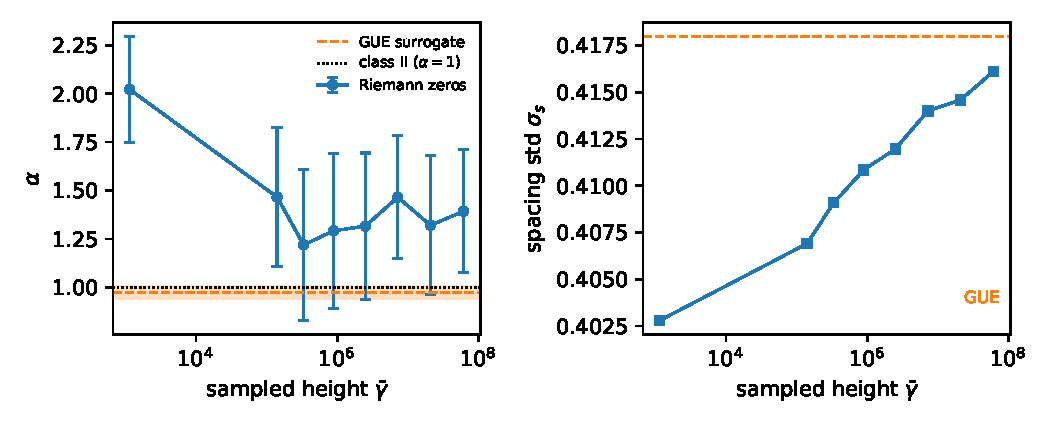
\includegraphics[width=\columnwidth]{../figures/fig3_alpha_vs_height.pdf}
\caption{Finite-height statistics of lattice-mapped Riemann-zero sequences,
from eight disjoint windows of $24\times5352$ zeros each. Left: hyperuniformity
exponent $\alpha$ versus sampled height $\bar\gamma$, with the GUE surrogate
(dashed, shaded band) and the class~II value $\alpha=1$ (dotted). The weighted
mean is $\alpha=1.49\pm0.12$, but $\alpha$ shows no height dependence: the
fitted slope is $-0.138\pm0.075$ ($1.8\sigma$), it is carried entirely by the
lowest window, and the upper seven points are flat
($+0.013\pm0.149$, $\chi^{2}/\mathrm{dof}=0.07$ about
$\alpha=1.364\pm0.135$). Right: nearest-neighbour spacing dispersion
$\sigma_s$ over the same windows, rising monotonically in all eight and
extrapolating to the GUE value near $\bar\gamma\sim10^{8.4}$. The short-range
rigidity drifts with height; the $k\to0$ exponent does not.}
\label{fig:height}
\end{figure}

A second systematic deserves note. Enforcing a target composition by flipping
a fraction $f$ of sites at random superposes a white component of relative
size $\sim f/[c(1-c)]$ on $s(k)$; on a class~I sequence $f\sim10^{-3}$ already
suffices to measure $\alpha\approx0$. Every generator must therefore reach the
target composition by construction.

\subsection{Transport observables}

For each transverse wavevector $k_\parallel^{(m)}$ an effective
one-dimensional chain is constructed, retaining all interlayer and
further-neighbor force constants without truncation. The implementation of every step below, including the Riemann--Siegel zero finder used for Eq.~\eqref{eq:unfold} and the window-disjointness constraint applied in Fig.~\ref{fig:height}, is available in the accompanying repository.

Three mutually redundant
routes are used: (i) the smallest Lyapunov exponent $\gamma(\omega)$ from
transfer-matrix products with periodic reorthogonalization, cost
$\mathcal{O}(N)$ and the cleanest route to the exponent of
Eq.~\eqref{eq:master}; (ii) recursive Green's function evaluation of the
Landauer transmission $\Tr(\omega)=\sum_m\Tr_m(\omega)$; and (iii) the kernel
polynomial method for $D(\omega)$, which also verifies that the class~II
sequence produces no spectral gaps---a negative result reported explicitly,
since gap formation requires Bragg peaks that a GUE-class sequence does not
possess.

\section{Proposed observable and design specifications}
\label{sec:observable}

\subsection{The differential measurement}

At low temperature the total relaxation rate decomposes by Matthiessen's rule,
\begin{equation}
  \frac{1}{\tau_{\rm tot}}
    = \underbrace{\frac{v}{L_{\rm eff}}}_{\rm Casimir}
    + \frac{1}{\tau_{\rm anh}(\omega,T)}
    + \frac{1}{\tau_{\rm def}(\omega)}
    + \frac{1}{\tau_{\rm iso}(\omega;s)} .
  \label{eq:matthiessen}
\end{equation}
Only the last term depends on the isotope \emph{arrangement}. The Casimir
boundary term~\cite{Casimir1938,Ziman1960} is frequency independent and exceeds the isotope term throughout the
sub-terahertz range, so any absolute measurement is background dominated.

Consider two samples carrying a class~II and a random arrangement, with
identical isotopic composition, geometry, surface preparation, growth batch,
and point-defect density. Their Hamiltonians then differ by a permutation of
masses alone; the first three terms of Eq.~\eqref{eq:matthiessen} are
identical term by term, and
\begin{equation}
  \Delta\!\left(\frac{1}{\tau}\right)
    = \frac{1}{\tau_{\rm iso}^{\rm rand}(\omega)}\big[1-\mathcal{R}(\omega)\big].
  \label{eq:diffrate}
\end{equation}

The composition-matching requirement is load bearing. A mismatch $\delta c$
produces a spurious difference in $g_2$; near $c=0.5$ the leading order
cancels but the second-order term still reaches the target effect for
$\delta c\sim1\%$. Compositions must be matched to $\delta c<0.2\%$, verified
by secondary-ion mass spectrometry and independently by the Raman $E_{2g}$
position, which shifts from $1394$~cm$^{-1}$ in h-\tenB N to $1358$~cm$^{-1}$
in h-\elevenB N~\cite{Vuong2018}.

Transmission is not linear in the relaxation rate. With
$\Tr_m=(1+L/\Lambda_m)^{-1}$ and $\Lambda_m=v_m\tau_m$,
\begin{equation}
  \Delta\Tr(\omega)\simeq\sum_m \Tr_m^{2}\,\frac{L}{v_m}\,
    \frac{1}{\tau_{{\rm iso},m}^{\rm rand}}\big[1-\mathcal{R}(\omega)\big].
  \label{eq:dT}
\end{equation}
The background cancels from the signal but not from the sensitivity: the
prefactor $\Tr_m^{2}$ retains all background scattering, so the sample must
remain quasi-ballistic, $L\lesssim\Lambda_{\rm background}$.

\subsection{Transverse integration}

A natural objection is that integration over $k_\parallel$ washes out
one-dimensional sequence effects. For Cantor-set gaps in quasiperiodic
superlattices this is valid: gap positions migrate channel by channel and the
summed spectrum is smeared. For power-law scaling it is not. The angular
average of Eq.~\eqref{eq:angavg} \emph{is} the continuum-limit channel sum; it
preserves the exponent and modifies only the prefactor $2/(\alpha+2)$.
Exponents are scale invariants and are immune to channel averaging.

This is why we adopt a thick three-dimensional geometry rather than a
nanoribbon. Quantizing $k_\parallel$ is unnecessary here, and the edges
required to achieve it introduce diffuse boundary scattering scaling as
$\Delta^{2}\omega^{2}/vW$ (Appendix), which necessarily dominates
$\omega^{4+\alpha}$ at low frequency.

\subsection{Feasibility window}
\label{sec:feasibility}

Taking in-plane h-BN parameters $v\simeq2\times10^{4}$~m\,s$^{-1}$ and
$V_0=9.05$~\AA$^{3}$/atom. An equimolar \tenB/\elevenB\ boron sublattice has
$g_2^{\rm B}=2.245\times10^{-3}$, but only the boron projection of the phonon
eigenvector contributes: for long-wavelength acoustic modes
$|\bm e(\kappa)|^{2}=M_\kappa/\sum_{\kappa'}M_{\kappa'}$, giving a boron weight
$10.81/(10.81+14.01)=0.436$ and hence an effective
$g_2=0.436\times2.245\times10^{-3}=9.8\times10^{-4}\simeq1\times10^{-3}$.
With this,
$\tau_{\rm iso}^{-1}\simeq9.0\times10^{-47}\,\omega^{4}$~s$^{-1}$. Below
$\sim4$~K, Umklapp processes are frozen out and normal processes do not relax
momentum, so the background is Casimir limited. For $\ell=1.25$~nm
($f_0=v/2\ell=8$~THz) and $L=300\,\mu$m:

\begin{table}[t]
\caption{Feasibility of the differential observable at $T\lesssim4$~K for
$\ell=1.25$~nm and $L=300\,\mu$m.}
\label{tab:window}
\begin{ruledtabular}
\begin{tabular}{ccccc}
$f$ (THz) & $\tau_{\rm iso}^{-1}$ (s$^{-1}$) & $\tau_B/\tau_{\rm iso}$ &
$\mathcal{R}$ & $\Delta\tau_{\rm tot}^{-1}/\tau_{\rm tot}^{-1}$ \\
\colrule
4 & $3.6\times10^{7}$ & 0.53 & 0.50 & 17\% \\
5 & $8.8\times10^{7}$ & 1.3  & 0.63 & 21\% \\
6 & $1.8\times10^{8}$ & 2.7  & 0.75 & 18\% \\
7 & $3.4\times10^{8}$ & 5.0  & 0.88 & 10\% \\
8 & $5.8\times10^{8}$ & 8.6  & 1.00 & 0    \\
\end{tabular}
\end{ruledtabular}
\end{table}

The accessible window is $4$--$7$~THz, optimal near $5$--$6$~THz, with a
predicted differential signal $\Delta\Tr/\Tr\sim20\%$. Both edges squeeze each
other: the lower edge is set by the Casimir background, whose reduction
requires larger $L$ but is capped by the quasi-ballistic condition; the upper
edge is $f_0=v/2\ell$, whose increase requires smaller $\ell$ but is bounded
below by Eq.~\eqref{eq:designrule} and by the resolvability of the GUE spacing
distribution on the discrete lattice. The two constraints intersect at
$\ell\simeq1.25$~nm, which we adopt as the design specification.

These values assume in-plane propagation and modulation. Modulation along the
stacking axis is more accessible to layer-by-layer growth but carries
$v_c\simeq3.5\times10^{3}$~m\,s$^{-1}$, which shifts $f_0$ down by a factor
$\sim6$ and closes the overlap with the Casimir crossover.

\subsection{Fabrication specification}

The window requires isotopic placement at $1.25$~nm pitch over $300\,\mu$m:
approximately $2.4\times10^{5}$ independently specified modulation units. We
state plainly that no present h-BN growth technique meets this specification.
Precursor switching in MOCVD along the $c$ axis provides layer-level control
but coherent modulation lengths of order $1\,\mu$m; in-plane isotopic
patterning at nanometer resolution has no established route.

This paper is therefore a theory and design-specification study. Its
contributions are the scaling law of Eq.~\eqref{eq:master}, the stealthy
window theorem, the discretization bound of Eq.~\eqref{eq:designrule}, and the
quantitative delimitation of the observation window together with the growth
capability required to reach it. We regard explicit statement of that gap as
more useful than its concealment.

\section{Conclusion}

The spatial arrangement of isotopes, at fixed isotopic variance, is a genuine
and previously unused control parameter for phonon transport. Generalizing the
Tamura theory through the mass-fluctuation structure factor yields
$\tau_{\rm iso}^{-1}\propto\omega^{\,d+1+\alpha}$, in which the hyperuniformity
exponent contributes additively and independently of dimension. Mapping a GUE-class sequence onto a
\tenB/\elevenB\ modulation converts the Rayleigh $\omega^{4}$ into
$\omega^{5}$; sequences built from Riemann zeros at finite height are
more rigid still, with $\alpha=1.49\pm0.12$ independent of the height sampled,
and a correspondingly deeper suppression. For stealthy arrangements the golden-rule rate
vanishes identically below $vK/2$, defining a hard transparency window.

Hexagonal boron nitride is the natural host: its boron sublattice carries an
anomalously large natural mass disorder ($g_2\approx1.35\times10^{-3}$, some
eighteen times that of natural carbon) while its nitrogen sublattice is nearly
isotopically pure, and its force constants are strictly untouched by the
substitution.

\emph{Data availability.} All code, generated sequences, and the manuscript
source are openly available at
\url{https://github.com/Ruqing1963/hbn-hyperuniform-isotope}. The repository
reproduces every figure and every number quoted in Secs.~\ref{sec:methods} and
\ref{sec:observable} from a single primitive-cell force-constant calculation,
and includes the regression tests for the scaling exponents of
Eq.~\eqref{eq:master}.

\appendix
\section{Boundary roughness scaling}

With the Ziman specularity parameter $p(\omega)=\exp(-4q^{2}\Delta^{2})$ for
rms roughness $\Delta$, the diffuse boundary rate is
\begin{equation}
  \frac{1}{\tau_{\rm edge}}=\big[1-p(\omega)\big]\frac{v}{W}
  \;\xrightarrow{\;q\Delta\ll1\;}\;
  \frac{4\Delta^{2}}{vW}\,\omega^{2}.
  \label{eq:edge}
\end{equation}
Comparison with Eq.~\eqref{eq:master} shows that boundary scattering dominates
at low frequency whenever $d+1+\alpha>2$, i.e. always. Equating the two rates
gives the crossover width
\begin{equation}
  W_{\rm cross}=\frac{16\pi\Delta^{2}v^{2}}{V_0\,g_2\,\omega^{2}},
  \label{eq:wcross}
\end{equation}
which for $\Delta=0.5$~nm and $f=1$~THz is of order $10^{2}\,\mu$m. Any
geometry narrow enough to quantize $k_\parallel$ is boundary dominated by four
to six orders of magnitude, which excludes the nanoribbon route
quantitatively.

\bibliography{refs}

\end{document}
